\documentclass{article}

\usepackage{multicol}
\usepackage{enumitem}
\usepackage[english]{babel}
\usepackage{graphicx}

\graphicspath{{./}}

\newcommand{\classname}[1]{\texttt{#1}}

\begin{document}

	\begin{titlepage}
		\begin{center}
			\rule{12cm}{0.4pt} \\
			[0.25in]
			\huge{\bfseries Sky Wars Coursework Report} \\
			[2mm]
			\rule{12cm}{0.4pt} \\
			[0.25in]
			\textsc{Edinburgh Napier University}
			\textsc{Software Development 3 (SET09101)} \\
			[110mm]
		\end{center} 
		
		\begin{flushright}
				\textsc{\large Jack Anderson \\
				40208539@live.napier.ac.uk \\
				November 23, 2016 \\
				}
			\end{flushright}
	\end{titlepage}

  	\pagenumbering{arabic}
  	
	\begin{multicols}{2}
  		
  		\section{Introduction}
  			The aim of this project was to create an implementation of the game 'Sky Wars' using Java, in order to demonstrate specific design patterns. 'Sky Wars' is a game which consists of a grid in which spaceships move randomly each to turn to any adjacent grid position. Each turn there is a chance that a new enemy will spawn in the top left hand corner of the grid. If the players ship lands on a grid position that contains enemies, what happens depends on the operational mode of the ship. When the ship is in defensive mode, if there is a single enemy it is destroyed. However, if there are two or more enemies the player is destroyed and the game ends. When the player is in aggressive mode, it takes three or more ships for the player to be destroyed.
  		\section{Patterns}
  		\paragraph{Command}
  			Several command objects exist which encapsulate all data needed to perform an action. All of these commands implement an execute and unexecute method which allows the action to be performed and reverted at any time. These commands are created and then stored inside a \classname{GameState} object which contains a list of actions performed for a single turn of the game. The \classname{GameState} then executes all commands stored inside of it, and is then added to a stack. This stack provides the ability to undo turns in the game by popping the last \classname{GameState} from the stack and unexecuting all of the commands which were performed, reverting the player back to the previous turn. Once the \classname{GameState} has been undone it is added to the Re-do stack. This stack provided the functionality to re-do a previously undone state, by simply executing all commands in the GameState.
  		\paragraph{Factory}
  			When a new movement is required, a \classname{MoveCommandFactory} is used. As the movement in the game is random, every time a \classname{MoveCommand} is to be created a random direction needs to be produced. The \classname{MoveCommandFactory} class takes in any \classname{SpaceShip}, generates a random direction which is valid, i.e. it does not move you off of the grid, and then creates and returns a new \classname{MoveCommand} object. 
  		\paragraph{Observer}
  			The \classname{SkyWarsCore} implements the \classname{IObservable} interface, and the main GUI class \classname{SkyWarsGame} implements the \classname{IObserver} interface. This allows the \classname{SkyWarsCore} class to register objects using the \classname{IObserver} interface as observers. This allows the \classname{SkyWarsCore} to notify the \classname{SkyWarsGame} when certain events take place. Notifications are sent to the \classname{SkyWarsGame} GUI when:
  			\begin{itemize}[noitemsep]
  				\item the game begins
				\item an enemy spawns
				\item an enemy is defeated
				\item the player is defeated
				\item the game ends
			\end{itemize}
			When \classname{SkyWarsGame} receives an update it writes the text supplied to it into a text area, allowing the player to see a history of events which have taken place in the game.
  		\paragraph{Strategy}
  			The strategy pattern is used to determine the outcome of combat within the game. The player ship contains reference to a strategy implementing the interface \classname{OperationalMode}. When the ships 'Combat' method is called, the implementation of this method is decided at runtime by using the 'Combat' method implemented in the ships \classname{OperationalMode}. This allows the ship to react differently to combat situations depending on its set \classname{OperationalMode}. Currently there are only two Operational Modes; \classname{DefensiveMode}, and \classname{OffensiveMode}, although this could easily be expanded to allow for different types of combat.
  		\section{Threads}
  			\paragraph{Threads} When the game is started a thread is started which redraws the panel containing the game a certain number of times every second depending on the framerate which was set. This allows additional game logic to carry out in the background, and the display is automatically updated to reflect the changes. Threading is also used to play sounds. Whenever certain events happen, e.g. an enemy is destroyed, a thread is started which plays a specified sound file for its entire duration. A thread is required so that the operation of the game logic is not halted while the sound file plays.
  
  	\end{multicols}
  	
	\newpage  	
  	
  	\section{GUI}
  	The GUI for Sky Wars contains a main game board on the left hand side displaying the current state of the game and several buttons. The 'Start Game' button begins a new game if not already started. The 'Move' button carries out a single turn in the game. The 'Undo' button reverts back to the previous game state, if one exits. The 'Redo' button reverts the game state back to before an undo had taken place, if the last action was an undo. The 'End Game' button clears the board, all game states, and stops the game. The two radio buttons 'Defensive' and 'Offensive' are used to switch the operational mode of the players ship during game play. There is also a text area at the bottom of the window which contains a list of events which have taken place during the game.
  		\begin{figure}[h]
  			\begin{center}
  				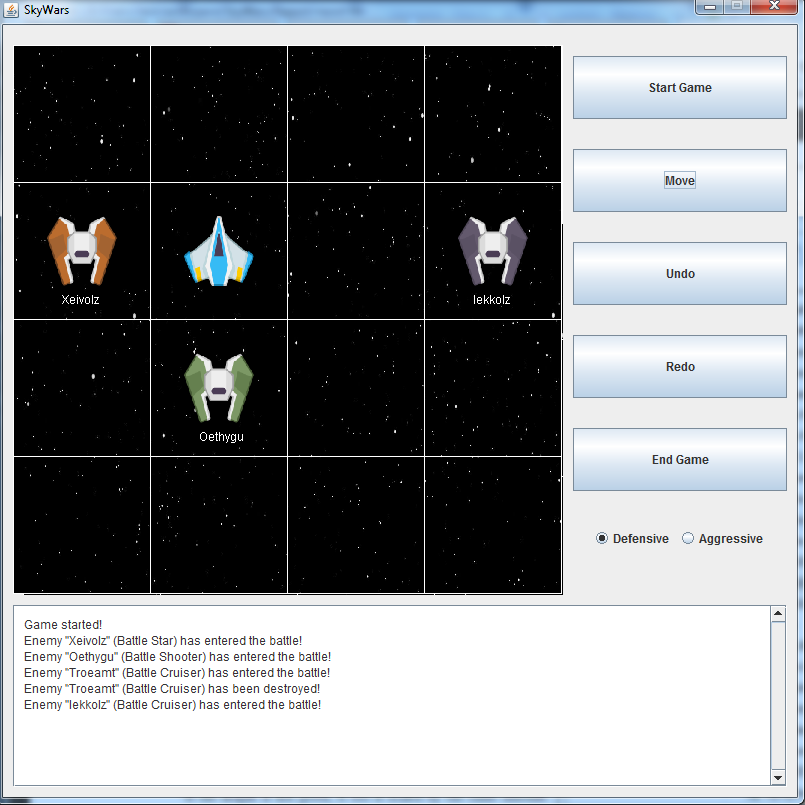
\includegraphics[width=.9\textwidth]{guiscreenshot}
  				\caption{Screenshot of the Sky Wars GUI}
  			\end{center}
  		\end{figure}
    \section{Class Diagram}
    	\begin{figure}[h]
  				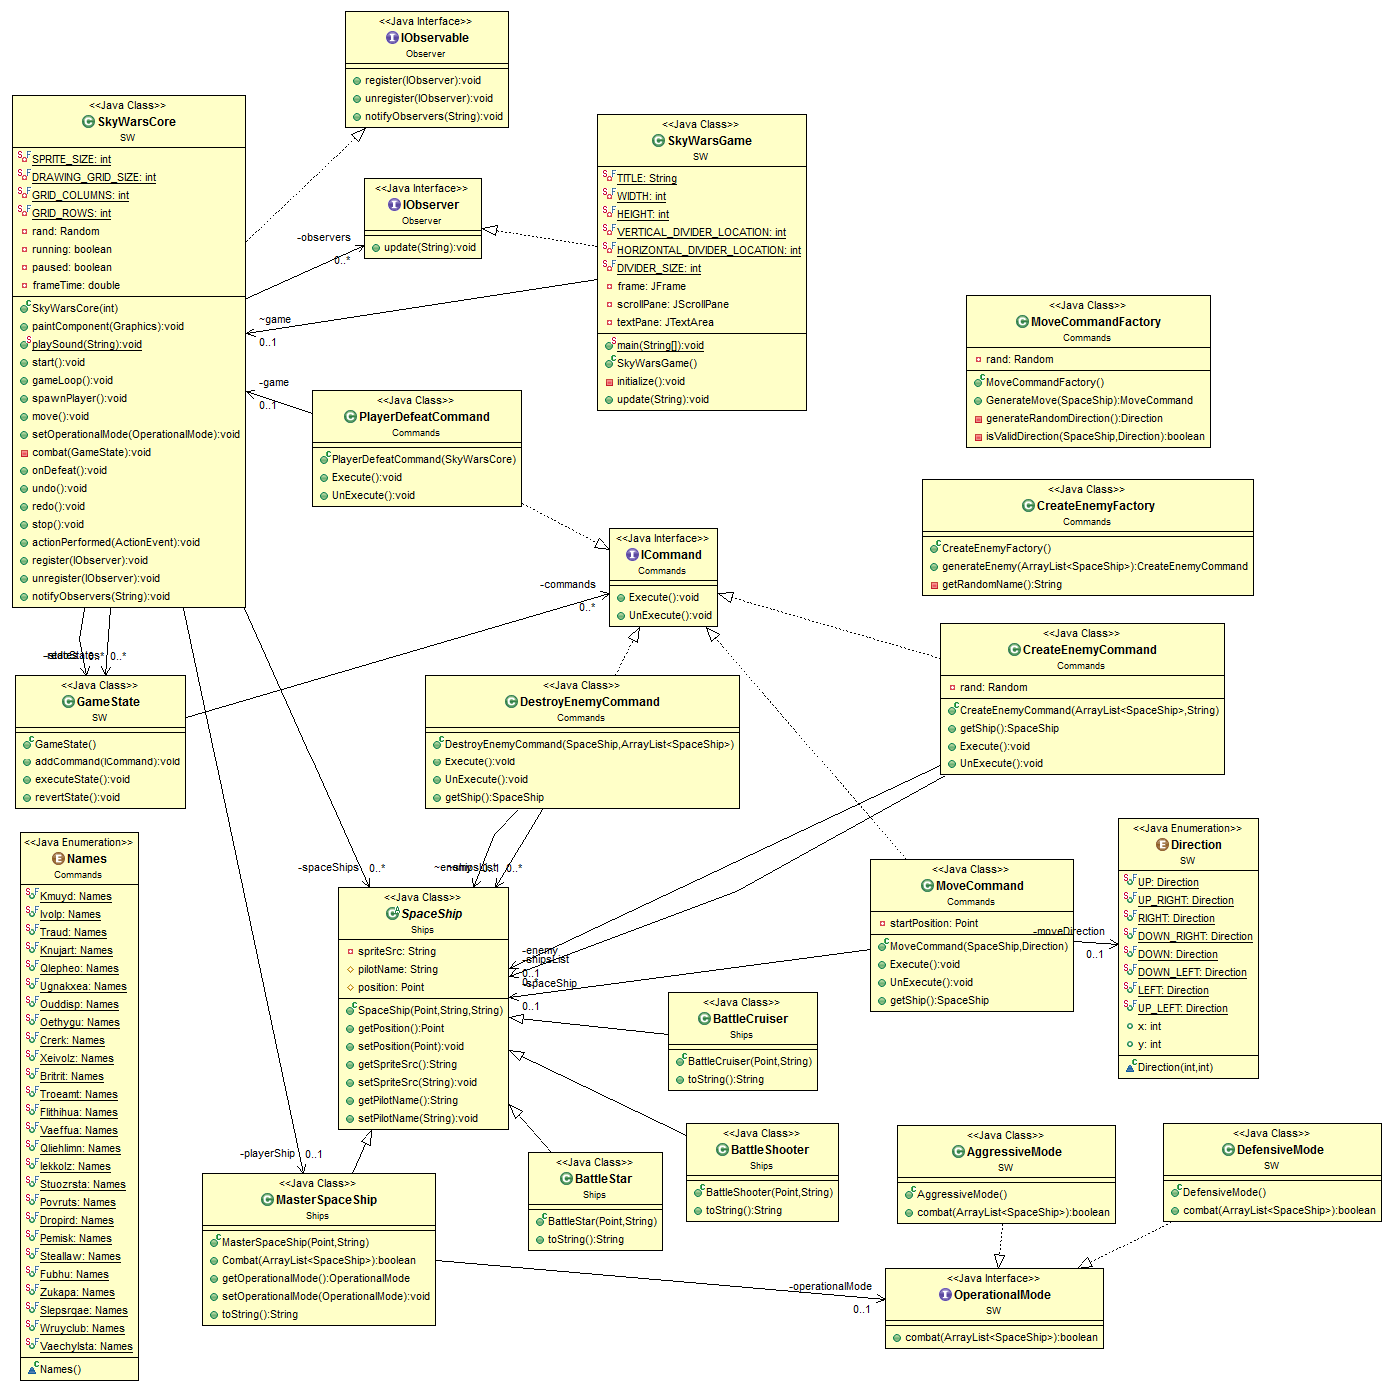
\includegraphics[scale=0.35]{classdiagram}
  				\caption{Sky Wars class diagram}
  		\end{figure}
\end{document}